\chapter{A telefonos alkalmazás fejlesztés}

A bevezetőben említett probléma nem újkeletű, a MOHOSZ tisztában van a horgász fogási napló digitalizálásával
kapcsolatos felmerülő igényekkel, több próbálkozás is volt már, mindent átfogó megoldás azonban eddig még nem valósult meg, csak tervek vannak terítéken\cite{Mohosz}.

A telefonos alkalmazások fejlesztésére több különböző módszer is létezik, ebben a fejezetben szeretném
ezt részletesebben bemutatni.

\section{Különböző szoftverek bemutatása}

A telefonos applikációk fejlesztésére többféle platformon elérhető szoftverek léteznek.
Továbbiakban ismertetni szeretném a kifejezetten számítógépes platformra készített népszerűbb programokat,
amelyek a telefonos alkalmazás fejlesztést hivatottak megkönnyíteni.
\vspace{.5cm}

Az egyik legnépszerűbb választás a Flutter, ami a felhasználó számára lehetővé teszi, hogy egyszerre
fejlesszenek a két legnagyobb telefonos platformra, azaz Android-ra , és IOS-re (továbbiákban Cross-platform).
Ez egy DART keretrendszeralapú ˝widget˝ fejlszetést kínál, aminek az előnye a gyors User Interface készítés,
és széleskörű testreszabhatóság\cite{Flutter}. Készítője a Google.

\begin{figure}[h]
\centering

\includegraphics[scale=0.2]{images/flutter.png}
\caption{Flutter logó}
\label{fig:flutter}
\end{figure}

A másik népszerű választás a React Native\cite{React}, amely szintúgy egy Cross-platform alkalmazás készítő szoftver,
amelyet a Facebook fejlesztett ki. A program JavaScript, illetve TypeScript programnyelvet használ,
nagy hangsúlyt fektet a gyorsaságra.

\begin{figure}[h]
\centering

\includegraphics[scale=0.1]{images/reactnative.png}
\caption{React Native logó}
\label{fig:reactnative}
\end{figure}

Említésre méltó a Unity\cite{Unity}, amely kifejezetten játék fejlesztésre készült szoftver.
Többek között képes számítógépes, konzolos és telefonos alkalmazás fejlesztésre is.
Fejlesztési nyelve a C\#.

\begin{figure}[h]
\centering

\includegraphics[scale=0.12]{images/unity.png}
\caption{Unity logó}
\label{fig:unity}
\end{figure}

A következő alkalmazás az Xcode\cite{Xcode}, amely az Apple hivatalos fejlesztői környezete.
Ezzel a szoftverrel csak az Apple ökoszisztémán létező operációs rendszerekre tudunk fejleszteni,
azaz iOS, iPadOS, macOS, watchOS és tvOS. Fejlesztési nyelve a Swift, és Objective C.

\begin{figure}[h]
\centering
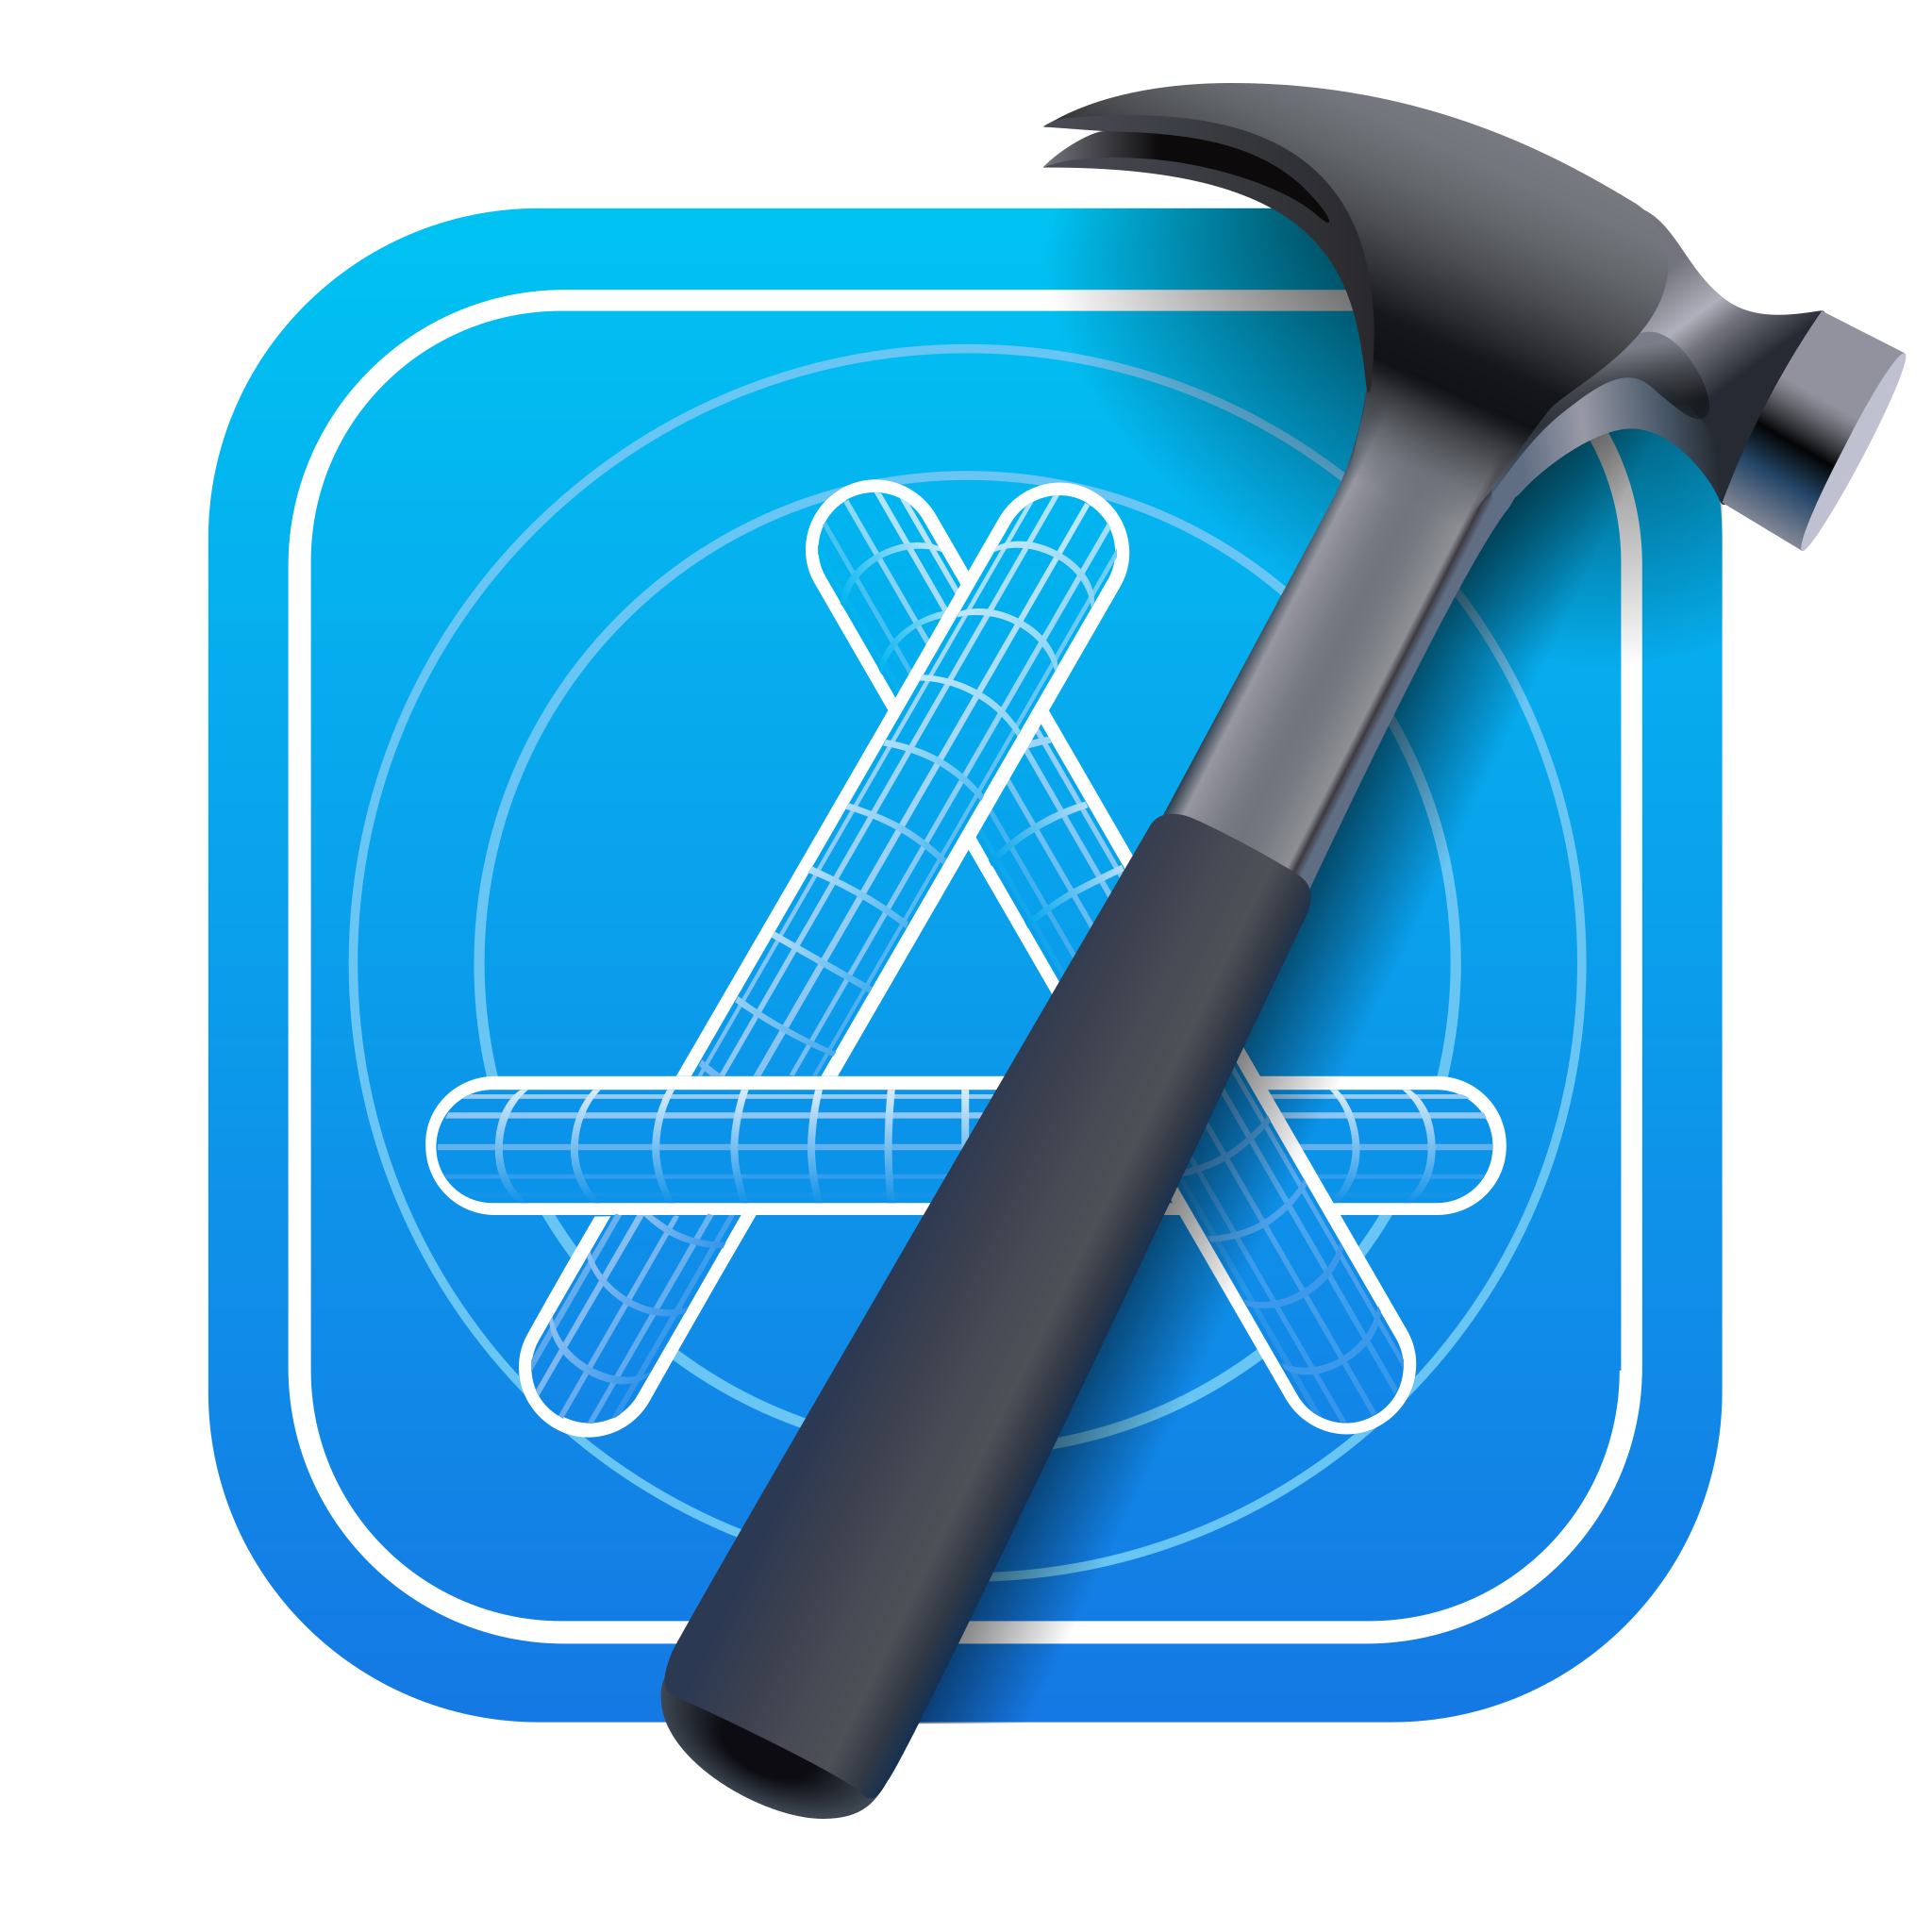
\includegraphics[scale=0.08]{images/xcode.png}
\caption{Xcode logó}
\label{fig:xcode}
\end{figure}

Utoljára pedig az általam választott szoftvert mutatnám be röviden, az Android Studio-t\cite{AndroidStudio}.
Ez a Google által fejlesztett hivatalos fejlesztő környezet, amellyel Andoridos alkalmazások
készítését teszik elérhetővé. Ez egy teljeskörő eszközkészlet, rendelkezik Android SDK-val, és 
beépített emulátorral, ami megkönnyíti a gyors tesztelést. Fejlesztési nyelve elsősorban a Kotlin, és a Java.

\begin{figure}[h]
\centering

\includegraphics[scale=0.08]{images/androidstudio.png}
\caption{Android Studio logó}
\label{fig:androidstudio}
\end{figure}

Az előbbiekben felsorolt fejlesztői környezeteknek nagyon sok előnye, és hátránya van. 
Az általam megadott szempontok a következők voltak: 
\begin{itemize}
    \item Androidon futtatható legyen az alkalmazás, hozzám közelebb áll a platform szemlélete a nyílt forráskódú applikációk terén.
    \item A fejlesztő környezet által használt nyelv sem elhanyagolható. Szerettem volna, ha egy magas szintű programozási nyelv lenne a használt az adott környezetben, tekintve hogy azokban szereztem a legtöbb tapasztalatom.
    \item Fontos volt a beépített emulátor, hogy az alkalmazásomat minél gyorsabban tudjam tesztelni.
    \item Nem utolsó sorban szerettem volna, ha az általam választott API-kat minél gördülékenyebben tudomm integrálni.
\end{itemize}

Ezen szempontok alapján haladva úgy döntöttem, hogy az Android Studio lesz számomra a legmegfelelőbb választás.

\section{Az Android Studio részletezése}

Az Android Studio a Google által készített hivatalos fejlesztőkörnyezet, amellyel natív 
Android alkalmazásokat tudunk készíteni.
A környezet a JetBrains IntelliJ IDEA\cite{Jetbrains} alapjaira épül, ebből lett tovább fejlesztve az Android platformra történő alkalmazások fejlesztésére.
Az Androidos platformon ez a legjellemzőbben használt IDE.


\begin{figure}[h]
\centering

\includegraphics[scale=0.08]{images/androiddev.png}
\caption{Android Developers logó}
\label{fig:androiddevelopers}
\end{figure}

Az Android Studio főbb funkciói, és jellemzői:
\begin{itemize}
    \item \textbf{Emulator:} A beépített emulátorral\cite{Emulator} a fejlesztés során gyorsan ki lehet próbálni az alkalmazáson eszközölt változtatásokat. Ezenkívül az emulatorral beállíthatjuk
    a tesztelni kívánt Android verziót, illetve készüléket, ezáltal tesztelni tudjuk alkalmazásunkat
    különböző verziószámú operációs rendszereken.
    \item \textbf{Build System (Gradle):} Az Android Studio Gradle-t\cite{Gradle} használ építési 
    rendszerként, amely megkönnyíti az alkalmazások automatizált építését és kezelheti a 
    különböző verziókat, függőségeket. A Gradle segítségével lehetőségünk van különböző
    buildek létrehozására, ami kulcsfontosságú volt a fejlesztés egyes fázisaiban.
    \item \textbf{Integrált hibakeresés és teljesítményelemzés:} A fejlesztői környezet lehetővé teszi, hogy könnyen diagnosztizáljuk és kijavítsuk az alkalmazásunk problémáit.
    Különféle eszközökkel, például CPU és memóriafigyelőkkel segít abban, hogy optimalizáljuk az alkalmazás teljesítményét.
    \item \textbf{Firebase és egyéb felhőszolgáltatások támogatása:} 
    Az Android Studio integrációt biztosít a Google Firebase platformmal\cite{Firebase}, ami megkönnyíti az
    adatbázisok, hitelesítés, felhasználói elemzések, értesítések és más felhőszolgáltatások 
    beépítését az alkalmazásba. Ez volt a legfontosabb szempont számomra, mivel az alkalmazásom több ponton is támaszkodik ezekre az API-kra.
    \item \textbf{Aktív közösség és támogatás:} A Google rendszeresen frissíti az Android Studiot, és nagy fejlesztői közösség\cite{AndroidDevGroup} is támogatja, ahol gyorsan választ kaphatunk a kérdéseinkre.
\end{itemize}

\section{Androidos alkalmazás fejlesztés}

Az előbbiekben részleteztem pár szempontot a fejlesztői környezettel kapcsolatban, azonban nem szeretném kihagyni azt sem, hogy milyen előnyei vannak az erre a platformra való fejlesztésnek közvetlenül.
A specifikus platform kiválasztás előnyei:
\begin{itemize}
    \item \textbf{Felhasználók aránya:} Magyarországon az Android operációs rendszerrel rendelkező eszközök piaci részesedése eléri a 80\% több független forrás szerint is.\cite{statistic1}\cite{statistic2}
    \item \textbf{Nyílt forráskód:} Az Android egy nyitottabb ökoszisztéma\cite{aosp}, nagyobb szabadságot kap a fejlesztő az alkalmazás funkcionalitásának, és megjelenítésének létrehozásában.
    \item \textbf{Költségek:} Az alkalmazás fejlesztése, feltéve hogy mi csinálunk mindent, nem kerül pénzbe. Ezalól nem kivétel a fejlesztői környezet használata, alkalmazásunk elérhetővé tétele, és karbantartása sem.
    \item \textbf{Pulikálás:} Az elkészült Androidos alkalmazást sokkal könnyebben tudjuk publikálni különböző áruházakban\cite{fdroid}, nem vagyunk rákényszerítve a telefon gyári alkalmazás áruházára.
\end{itemize}

Az Android platform legfőbb hátránya:

\begin{itemize}
    \item \textbf{Fragmentáció, kompatibilitási problémák:} Legfőbb hátránya a platformnak a megszámolhatatlan mennyiségű hardver, és képernyőméret kombinációk. Ezáltal alkalmazásunk fejlesztésekor nagy valószínűséggel gyártunk olyan hibákat, amelyek láthatatlanok voltak számunkra. Ezentúl különböző Android verziók eltérőek lehetnek mind funkciókban, és használható API-kban. Ezáltal a fejlesztés elhúzódhat, mivel a lehető legtöbb készüléket kell lefednünk az alkalmazásunkal, ami időigényes.
\end{itemize}
